\documentclass{article}
\usepackage[utf8]{inputenc}
\usepackage{amsmath}
\usepackage{amsfonts}
\usepackage{amsthm}
\usepackage{parskip}
\setlength{\parindent}{0em}
\setlength{\parskip}{1em}
\usepackage{datetime}
\usepackage{algpseudocode}
\usepackage{graphicx}
\usepackage[
	citestyle=ieee, 
    bibstyle=ieee,
    style=numeric-comp,
    sorting=nty,
    maxbibnames=99, % Make sure we are printing all authors in the appendix
]{biblatex}
\addbibresource{references.bib}
\usepackage{caption}
\usepackage{subcaption}
\usepackage{pgffor} % Allows using foreach
\usepackage[section]{placeins} % Avoids placing floats before section

\newdateformat{monthyeardate}{%
  \monthname[\THEMONTH], \THEYEAR}

\title{Complex and Social Networks \\ Assignment 2 - Analysis of the degree distribution}
\author{Daniel Benedí García\\ José Ángel Vicente Porres}
\date{\monthyeardate\today}

\begin{document}
\maketitle

\section{Introduction}
This study initiates an investigation into the analysis of degree distributions within the global syntactic dependency networks of various languages. These networks serve as depictions of linguistic structures, where individual vertices are associated with lexical units, specifically words, while edges signify syntactic relationships, ascertained through their occurrence in dependency treebanks. Our research is primarily directed towards the examination of in-degree distributions, which provide valuable perspectives on the prevalence and structural arrangement of incoming syntactic dependencies within these intricate linguistic networks.

The primary aim of this study is to infer the underlying rules governing the observed degree distributions. To achieve this objective, the central focus will involve a comparative analysis between the empirical in-degree distributions and a predefined set of mathematical models. To ascertain the best possible fit to the observed data, we will employ the Maximum Likelihood Estimation (MLE) technique, which will aid in determining which model(s) most accurately capture the distribution patterns observed in the linguistic networks under investigation. This analytical approach will facilitate a deeper understanding of the organizational principles governing syntactic dependencies within diverse languages.

\section{Results}
In computational linguistics, various mathematical models are employed to represent the distribution patterns of in-degree within syntactic graphs for different languages. Commonly analyzed distributions include displaced Poisson, displaced geometric, zeta, truncated zeta, and Altmann distribution (also known as Menzerath's law) \cite{altmann1980prolegomena}.

Each distribution is characterized by specific parameters that require adjustment to achieve an optimal fit with the given dataset. The methodology employed for parameter estimation is maximum likelihood estimation, as elaborated in Section \ref{sec:mle}. To assess and compare the goodness of fit for different distributions, we utilize the Akaike information criterion (AIC) \cite{Akaike1998}. Herein, we define $AIC_{best}$ as the minimum AIC across all models. Consequently, for each model $m$, we calculate $\Delta AIC_m = AIC_m - AIC_{best}$, aiming to identify the model that best approximates our data. In Table \ref{tab:aic}, we present the $\Delta AIC$ values for each model in every language, where values closer to 0 indicate a stronger alignment with our optimal approximation.

\begin{table}[!htb]
\centering
\resizebox{\columnwidth}{!}{
\begin{tabular}{llllllllllll}
Language & 0 & 1 & 2 & 3 & 4 & 5 & 1+ & 2+ & 3+ & 4+ & 5+ \\ \hline

 Arabic & 1090.844 & 348.789 & 343.564 & 337.472 & 364.490 & 335.264 & 346.055 & 337.043 & 336.620 & 361.473 & 360.419 \\
 Basque & 276.863 & 59.999 & 60.872 & 70.595 & 67.913 & 62.666 & 61.012 & 62.701 & 118.112 & 68.111 & 64.666 \\
 Catalan & 814.121 & 110.801 & 108.285 & 120.996 & 135.333 & 103.241 & 109.350 & 106.574 & 134.331 & 132.297 & 153.161 \\
 Chinese & 274.712 & 126.245 & 125.080 & 119.838 & 131.616 & 121.833 & 126.102 & 123.254 & 121.014 & 131.641 & 141.704 \\
 Czech & 723.596 & 517.324 & 505.521 & 516.025 & 528.527 & 508.621 & 511.453 & 507.224 & 508.202 & 524.104 & 519.399 \\
 English & 724.102 & 219.578 & 221.388 & 245.239 & 243.884 & 222.683 & 221.509 & 222.513 & 317.254 & 237.543 & 224.499 \\
 Greek & 711.355 & 221.851 & 222.721 & 230.065 & 227.511 & 224.541 & 222.881 & 224.493 & 240.015 & 227.840 & 226.488 \\
 Hungarian & 610.872 & 203.171 & 204.834 & 248.298 & 275.524 & 206.772 & 204.811 & 206.811 & 279.376 & 240.936 & 208.752 \\
 Italian & 705.677 & 199.994 & 194.329 & 203.435 & 215.157 & 192.881 & 196.287 & 192.775 & 220.399 & 211.555 & 194.727 \\
 Turkish & 412.776 & 54.528 & 56.489 & 87.728 & 61.155 & 55.821 & 56.420 & 57.479 & 148.680 & 60.547 & 56.832 \\
\end{tabular}}
\caption{Akaike information criterion (AIC) of each model \label{tab:aic}}
\end{table}


Table \ref{tab:aic} presents a compelling argument, demonstrating that in the majority of cases, Altmann's distribution emerges as the optimal choice due to its consistently lowest AIC values. This assertion is further supported by a visual examination of the fit depicted in Figure \ref{fig:cat_fit}, where the Altmann distribution closely aligns with the observed data, substantiating its efficacy as an approximation.

Turning our attention to the Hungarian language dataset, as depicted in Figure \ref{fig:hun_fit}, the $\Delta AIC$ criterion favors the selection of the zeta distribution over the truncated zeta or Altmann distributions. Although both truncated zeta and Altmann distributions exhibit commendably close $\Delta AIC$ values, the consideration of AIC's definition elucidates that these distributions had lower likelihoods due to their additional parameters. This outcome stems from AIC's penalty mechanism, wherein each extra parameter incurs a penalty of 2, and both truncated zeta and Altmann distributions possess one extra parameter compared to the zeta distribution.

By adopting the zeta distribution with $\gamma = 2$ as the baseline, a graphical comparison in Figure \ref{fig:cat_fit} and \ref{fig:hun_fit} unequivocally underscores the inadequacy of the displaced Poisson and displaced geometric distributions as approximations for our data. Conversely, the fitted zeta distribution, the truncated variant, and the Altmann distribution stand out as highly effective approximations, closely matching the observed data in stark contrast to the zeta distribution with $\gamma = 2$. This behaviour can be observed in all the figures of appendix \ref{sec:fit_figures}.

\begin{figure}[h]
    \centering 
    \begin{subfigure}[b]{0.44\textwidth}
         \centering
         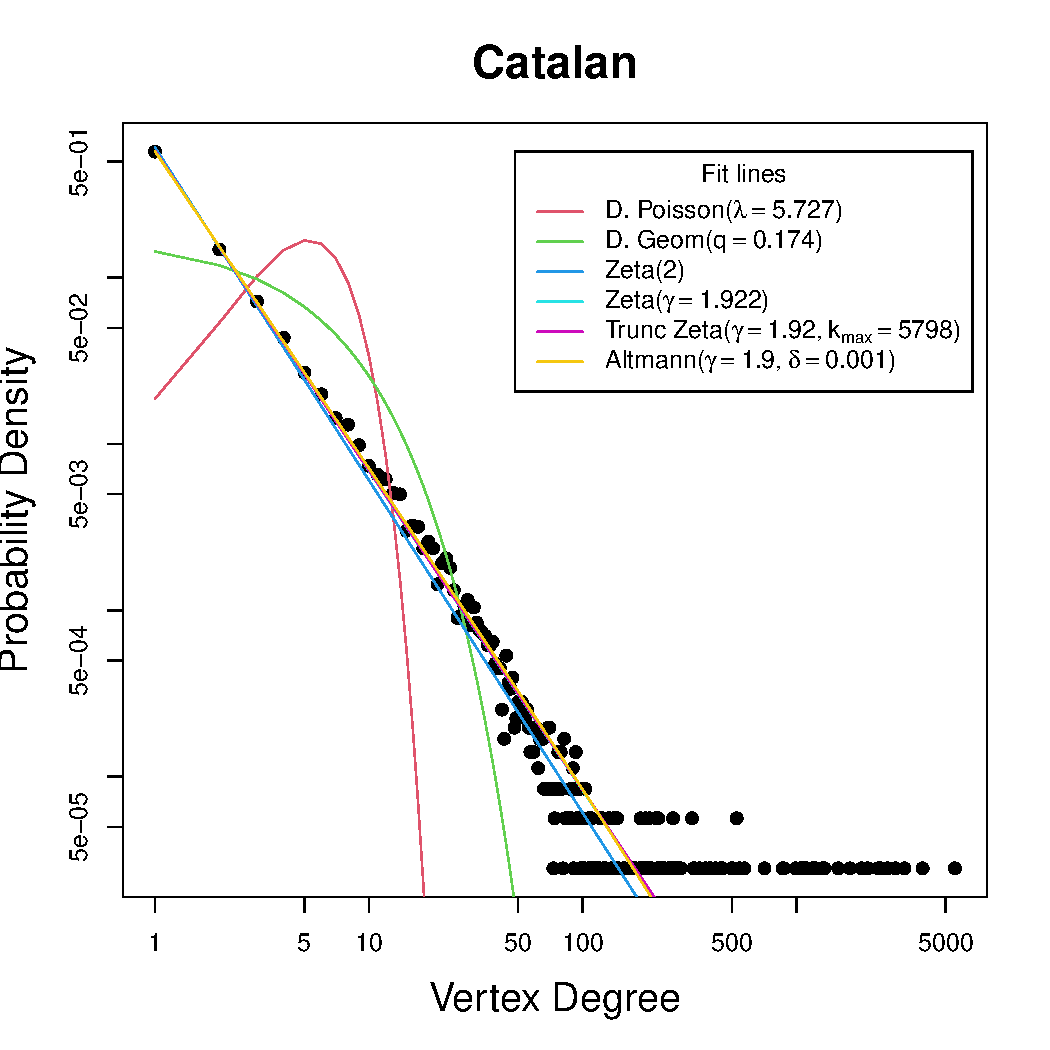
\includegraphics[width=\textwidth]{figures/Catalan_fit.pdf}
         \caption{Comparison of distributions for Catalan}
        \label{fig:cat_fit}
     \end{subfigure}
     \hfill
    \begin{subfigure}[b]{0.44\textwidth}
         \centering
         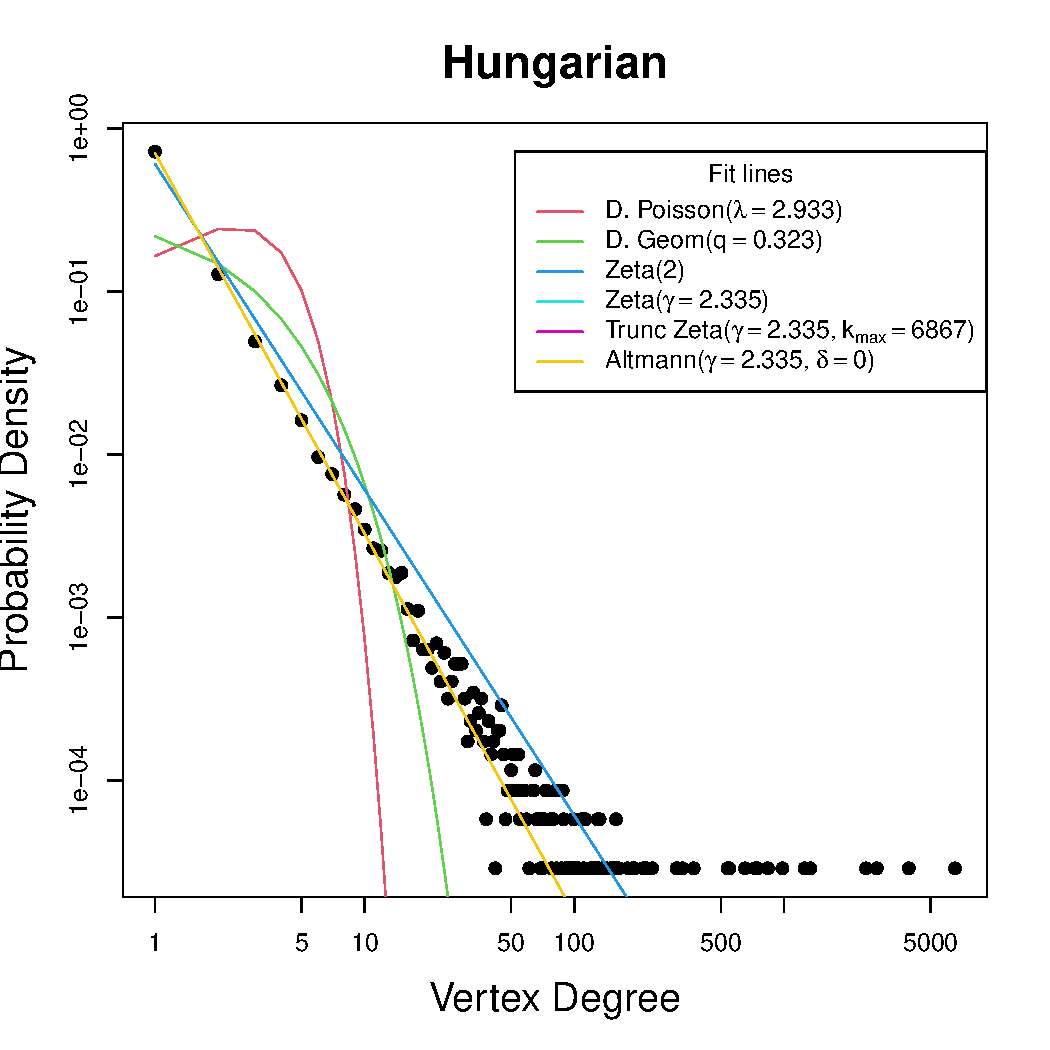
\includegraphics[width=\textwidth]{figures/Hungarian_fit.pdf}
         \caption{Comparison of distributions for Hungarian}
         \label{fig:hun_fit}
     \end{subfigure}
     \caption{Distributions fitted for  some example languages}
\end{figure}

\section{Discussion}

\subsection*{Log-log plots and precision of the empirical distributions}
In the analysis of the provided data sets, a consistent pattern emerges across all plots. For instances characterized by low degrees, the data points exhibit a distinctive arrangement, forming an exceedingly narrow and nearly linear alignment. Nevertheless, as one progresses along the distribution towards higher degrees, a transformation occurs, leading to the gradual broadening and decreased precision of this linear alignment. Eventually, at the extreme right end of the distribution, the data points adopt a nearly horizontal orientation. 

It is imperative to acknowledge the utilization of a log-log scale, where each unit of grid displacement results in exponential scale expansion. Natural plots have been omitted from presentation, as they fail to yield informative insights. However, it is important to realize that our findings are predicated upon a power-law distribution, necessitating careful consideration in the analysis of the obtained results.

In the examination of higher-degree points, an apparent trend emerges wherein the precision of their distribution appears to diminish progressively. This phenomenon can be attributed to the exponential reduction in the population of nodes. Consequently, even minute statistical uncertainties exert a substantial influence on the accuracy of individual points.

Around the terminal segment of the plot, we have to take into account the fundamental characteristics of empirical distributions. These distributions exhibit a limitation in precision, not surpassing a granularity of $1/N$, wherein $N$ denotes the sample size. The horizontal line depicted in the plot is result of this threshold, signifying not an actual proclivity of the distribution to persist in a horizontal trajectory, but rather the limitations imposed by small sample sizes for achieving a more refined portrayal of the underlying distribution.

\subsection*{Fitted lines}

While examining the graphical representations (appendix \ref{sec:fit_figures}), one may initially be inclined to hypothesize that the observed curves exhibit a sub-optimal fit to the distribution in the context of higher degrees. This apparent discrepancy can be attributed, once again, to the inherent imprecision of the empirical distribution as it approaches the upper extremities of the spectrum. We have to take into account, however, that both the likelihood function and the Maximum Likelihood Estimation (MLE) method do not succumb to this limitation in precision. These statistical techniques use direct information from the sample dataset, making predictions with greater accuracy and reliability. The parameters of the fitted  distributions can be observed in table \ref{tab:fitted}.

\begin{table}[!htb]
\centering
\begin{tabular}{llllllll}
\multicolumn{1}{r}{\textbf{}} & \multicolumn{5}{c}{\textbf{Model}} \\ \cline{2-8} 
\multicolumn{1}{c}{\textbf{}} &
  \multicolumn{1}{c}{D. Poisson} &
  \multicolumn{1}{c}{D. Geom} &
  \multicolumn{1}{c}{Zeta} &
  \multicolumn{2}{c}{Truncated Z} &
  \multicolumn{2}{c}{Altmann} \\
\multicolumn{1}{c}{\textbf{Language}} &
  \multicolumn{1}{c}{$\lambda$} &
  \multicolumn{1}{c}{$q$} &
  \multicolumn{1}{c}{$\gamma_1$} &
  \multicolumn{1}{c}{$\gamma_2$} &
  \multicolumn{1}{c}{$k_{max}$}  &
  \multicolumn{1}{c}{$\gamma_3$} &
  \multicolumn{1}{c}{$\delta$} \\ \hline
\multicolumn{1}{c}{Arabic} & 3.217 & 0.298 & 2.104 & 2.103 & 2361  & 2.086 & 0.001  \\
\multicolumn{1}{c}{Basque} & 1.831 & 0.459 & 2.358 & 2.357 & 605  & 2.347 & 0.002  \\
\multicolumn{1}{c}{Catalan} & 5.727 & 0.174 & 1.922 & 1.920 & 5798  & 1.900 & 0.001  \\
\multicolumn{1}{c}{Chinese} & 5.173 & 0.192 & 1.886 & 1.884 & 8027  & 1.835 & 0.003  \\
\multicolumn{1}{c}{Czech} & 3.891 & 0.252 & 2.051 & 2.050 & 4963  & 2.041 & 0.001  \\
\multicolumn{1}{c}{English} & 6.850 & 0.146 & 1.800 & 1.795 & 4774  & 1.740 & 0.003  \\
\multicolumn{1}{c}{Greek} & 3.407 & 0.284 & 2.132 & 2.130 & 1135  & 2.132 & 0.000  \\
\multicolumn{1}{c}{Hungarian} & 2.933 & 0.323 & 2.335 & 2.335 & 6867  & 2.335 & 0.000  \\
\multicolumn{1}{c}{Italian} & 4.165 & 0.236 & 2.108 & 2.107 & 2812  & 2.108 & 0.000  \\
\multicolumn{1}{c}{Turkish} & 2.000 & 0.432 & 2.543 & 2.543 & 7039  & 2.543 & 0.000  \\
\end{tabular}
\caption{Values of fitted parameters per distribution and language} \label{tab:fitted}
\end{table}

\section{Methods}

\subsection*{Degree distribution, understanding the plots}

The initial phase of this research project focused on ensuring the precise representation of the dataset. An overview of the utilized data is provided in Table \ref{tab:data}. Following the importation of the data points sequence, the generation of a frequency table, and the visualization of the outcomes, it became apparent that the resulting plots did not faithfully reflect the data. Specifically, certain nodes exhibited degrees exceeding a thousand, yet were inadequately represented in the generated plots. This discrepancy was attributed to the data factorization process conducted using the R command \verb|table|. To rectify this issue, we proceeded to transform the data into a \verb|data.set| format, allowing for better manipulation and accurate visual representations. The distribution plots are presented in the figures of Appendix \ref{append:spect} and \ref{append:spect_loglog}.

% latex table generated in R 4.3.2 by xtable 1.8-4 package
% Wed Nov 22 15:27:58 2023
\begin{table}[ht]
\centering
\begin{tabular}{lllll}
  \hline
Network & Vertices & Edges & Mean.Degree & Density \\ 
  \hline
Karate & 34 & 78 & 4.5882 & 0.139 \\ 
  Barabasi-Albert & 200 & 800 & 8 & 0.0402 \\ 
  ENRON & 182 & 2097 & 23.044 & 0.1273 \\ 
  DBLP & 2130 & 4587 & 4.307 & 0.002 \\ 
   \hline
\end{tabular}
\caption{Summary of the properties of the networks used.}
\label{tab:summary}
\end{table}


\subsection*{Zeta distribution and right truncation}

Due to a lack of precision, there is a tail at the end of the plots in the empirical distribution. Even though they do not affect the MLE method for fitting lines, we do not have any kind of information about how the data behaves in this area.

For this reason we propose the implementation of the right truncated zeta, by not taking into account the end points of the distribution.
$$
    TruncZ(k) = \begin{cases}
    \frac{1}{\sum_{x=1}^{k_{max}}x^{-\gamma}}k^{-\gamma}       & \quad \text{if } k \leq k_{max}\\
    0  & \quad \text{otherwise}
  \end{cases}
$$
However, MLE methods are not able to discern which is the optimal bound for this kind of models, because the likelihood function is monotonic on the $k_max$ parameter. Therefore, we opted to slowly ($1\%$ max degree) increase $k_max$ until the $-2\mathcal{L}$ converges in the sixth decimal place. The first value assigned to $k_max$ was the maximum degree because otherwise, we would have had points with probability 0 and therefore a likelihood of $log(0)$, which would have been a problem. Another possibility to could have been to assign a fixed value. 

\section{Maximum Likelihood Estimation \label{sec:mle}}
Maximum likelihood estimation (MLE) involves the process of determining the parameters of an assumed probability distribution based on observed data. It entails maximizing a likelihood function such that, within the context of the assumed statistical model, the observed data has the highest probability. It is defined as follow:
$$
\mathcal{L}(\text{params} | \mathbf{x} \text{, model}) = \sum_{i=1} \log{p(x_i \text{; params})}
$$

In the problem statement, the likelihood functions where given for some probability functions.
\begin{table}[!htb]
\resizebox{\columnwidth}{!}{
\begin{tabular}{lll}
 & Probability function & Likelihood function \\ \hline
 Displaced Poisson & $ p(k) = \lambda^k\frac{e^{-\lambda}}{k!(1-e^{-\lambda})} $ & $ \mathcal{L}(\lambda) = M \log \lambda - N(\lambda + \log(1-e^{-\lambda})) - C $ \\
 Displaced Geometric & $ p(k) = (1-q)^kq $ & $ \mathcal{L}(q) = (M - N)\log(1-q)+N\log q $ \\
 Zeta & $ p(k) = \frac{k^{-\gamma}}{ \zeta(\gamma) } $ & $ \mathcal{L}(\gamma) = -\gamma M' - N \log\zeta(\gamma) $ \\
 Truncated Zeta & $ p(k) = \begin{cases}
    \frac{1}{\sum_{x=1}^{k_{max}}x^{-\gamma}}k^{-\gamma} & \text{if } k \leq k_{max}\\
    0  & \text{otherwise}
  \end{cases} $ & $ \mathcal{L}(\gamma,k_max) = -\gamma M' - N \log \sum_{x=1}^{k_max}x^{-\gamma} $ \\
\end{tabular}}
\end{table}

Moreover, we used the Altmann distribution $p(k) = k^{-\gamma}e^{-\delta k}\frac{1}{\sum_{x=1}^Nx^{-\gamma}e^{-\delta x}}$, for which we had to derive its likelihood function:
\begin{align*}
    \mathcal{L}(\gamma, \delta) &= \sum_{i = 1} \log p(k_i) \\
    &= \sum_{i = 1} \log\left( k_i^{-\gamma}e^{-\delta k_i}\frac{1}{\sum_{x=1}^N x^{-\gamma}e^{-\delta x}} \right) \\
    &= \sum_{i = 1} \log(k_i^{-\gamma}) + \log(e^{-\delta k_i}) - \log(\sum_{x=1}^N x^{-\gamma}e^{-\delta x}) \\
    &= \sum_{i = 1} -\gamma\log{k_i} - \delta k_i - \log(d) \\
    &= - \gamma M' - \delta M - N \log(d)
\end{align*}

In order to maximize this likelihood we used the \verb|mle| method of the R package \verb|stats4|. We configured it to use Limited-memory Broyden–Fletcher–Goldfarb–Shannon bounded (L-BFGS-B). We opted to use L-BFGS-B because t allowed us to establish bounds which is not possible with other methods such as BFGS, CG (more fragile than the BFGS methods), SANN (only allows one dimensional parameters so we could not use it for Altmann) and showed a good performance.

\subsection*{Validation}
The hardest part of this kind of models, is to make sure that the methods used are in fact an effective representation of the data sample displayed. In this kind of cases, the simplest way is to get a sample known for following the distribution and study the fitting of the model. Here, in \ref{fig:val} we present the lines obtained at fitting the geometric and zeta MLE models over their respective empirical distributions for different parameters

\begin{figure}[!htb]
    \centering 
    \begin{subfigure}[b]{0.44\textwidth}
         \centering
         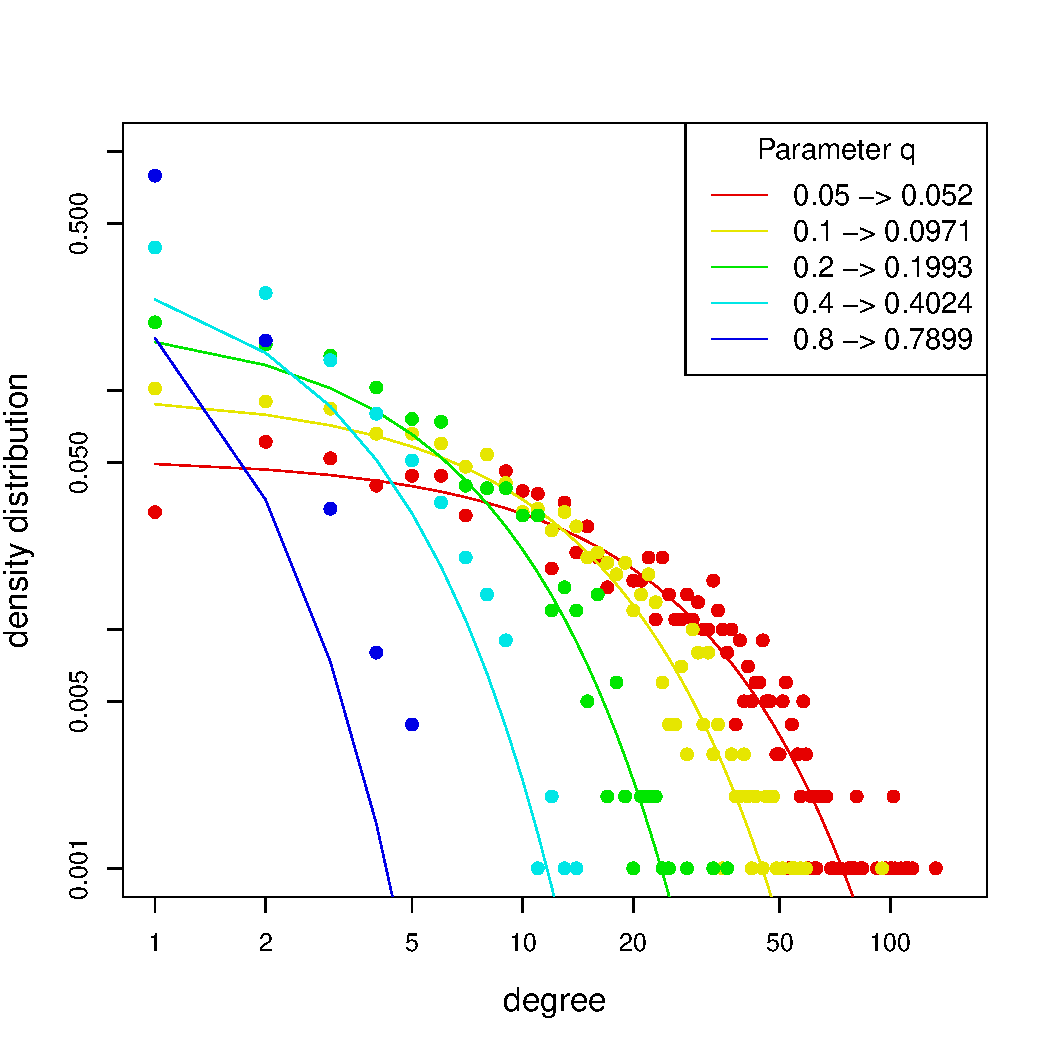
\includegraphics[width=\textwidth]{figures/geom_validation.pdf}
         \caption{Geometric distribution}
        \label{fig:geom_val}
     \end{subfigure}
     \hfill
    \begin{subfigure}[b]{0.44\textwidth}
         \centering
         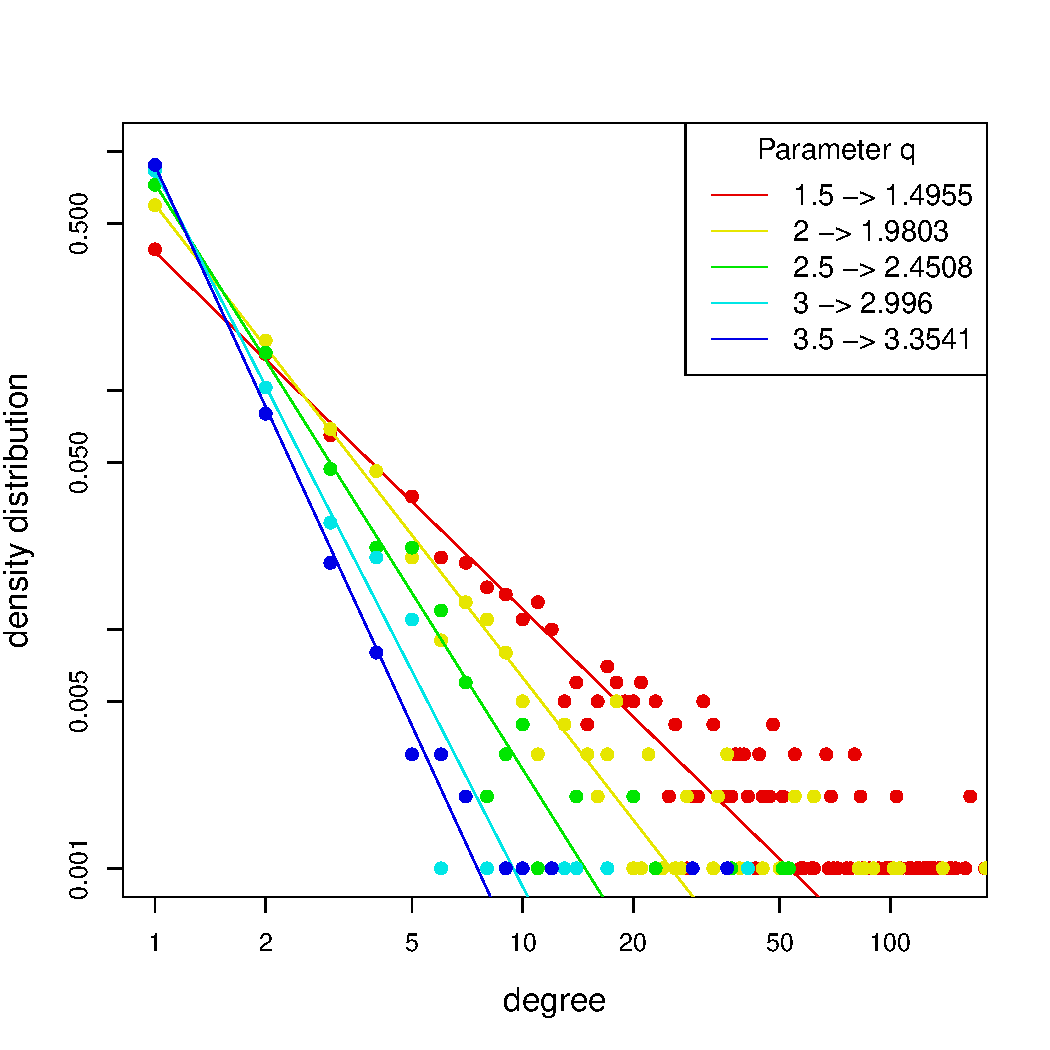
\includegraphics[width=\textwidth]{figures/zeta_validation.pdf}
         \caption{Zeta distribution}
         \label{fig:zeta_val}
     \end{subfigure}
     \caption{Validations fit for different distributions and parameters}
     \label{fig:val}
\end{figure}

We can observe, that in most cases, the model fit quite well the empirical distributions. However, it seems to fail in the geometric when the parameter tends to $1$. 

For this project, as we have seen in the discussion, the models that better fit our real samples are the ones similar to the zeta distribution. As we can see in \ref{fig:zeta_val}, this kind of models fit well in our experimental range. 

\addcontentsline{toc}{section}{References}
\printbibliography

\newpage
% Activate the appendix
% from now on sections are numerated with capital letters
\appendix
\def\Languages{
Arabic,
Basque,
Catalan,
Chinese,
Czech,
English,
Greek,
Hungarian,
Italian,
Turkish}

\section{Figures of the spectrum of each language  \label{append:spect}}
\foreach \lang in \Languages
{
\begin{figure}[!htb]
    \centering
    \includegraphics[width=0.7\textwidth]{figures/\lang_spectrum.pdf}
    \caption{Degree distribution spectrum of \lang}
\end{figure}
}
\pagebreak

\section{Figures of the spectrum of each language using log-log \label{append:spect_loglog}}
\foreach \lang in \Languages
{
\begin{figure}[!htb]
    \centering
    \includegraphics[width=0.7\textwidth]{figures/\lang_spectrum_loglog.pdf}
    \caption{Degree distribution spectrum of \lang}
\end{figure}
}

\pagebreak

\section{Figures with all the models fitted for each language \label{sec:fit_figures}}
\foreach \lang in \Languages
{
\begin{figure}[!htb]
    \centering
    \includegraphics[width=0.7\textwidth]{figures/\lang_fit.pdf}
    \caption{Fitted probability distributions for \lang}
\end{figure}
}

\end{document}
